\documentclass[10pt,twoside]{article}
\usepackage{etex, {soul}}
\newcommand{\num}{6{} }

\raggedbottom

%geometry (sets margin) and other useful packages
\usepackage{geometry}
\geometry{top=.8in, left=.8in,right=.8in,bottom=.8in}
 \usepackage{graphicx,booktabs,calc}

%=== GRAPHICS PATH ===========
\graphicspath{{./images/}}
% Marginpar width
%Marginpar width
\newcommand{\pts}[1]{\marginpar{ \small\hspace{0pt} \textit{[#1]} } }
\setlength{\marginparwidth}{.5in}
%\reversemarginpar
%\setlength{\marginparsep}{.02in}

%% Fonts
% \usepackage{fourier}
% \usepackage[T1]{pbsi}

\usepackage{lmodern}
\usepackage[T1]{fontenc}
%\usepackage{minted}

\usepackage{rotating}
%% Cite Title
\usepackage[style=authoryear,backend=biber, natbib,maxcitenames=2,doi=false,isbn=false,url=false,eprint=false]{biblatex}
\addbibresource{../Water-Accessibility.bib}

%%% Counters
\usepackage{chngcntr,mathtools}
\counterwithout{figure}{section}
\counterwithout{table}{section}

\numberwithin{equation}{section}

%% Captions
\usepackage{caption}
\captionsetup{
  labelsep=quad,
  justification=raggedright,
  labelfont=sc
}

%AMS-TeX packages
\usepackage{amssymb,amsmath,amsthm}
\usepackage{bm}
\usepackage[mathscr]{eucal}
\usepackage{colortbl}
\usepackage{color}


\usepackage{epstopdf,subfigure,hyperref,enumerate,polynom,polynomial}
\usepackage{multirow,minitoc,fancybox,array,multicol}

\definecolor{slblue}{rgb}{0,.3,.62}
\hypersetup{
    colorlinks,%
    citecolor=blue,%
    filecolor=blue,%
    linkcolor=blue,
    urlcolor=slblue
}

%%%TIKZ
\usepackage{tikz}
\usepackage{pgfplots}
\usepackage{pgfplotstable}
\usepackage{pgfgantt}
\pgfplotsset{compat=newest}

\usetikzlibrary{arrows,shapes,positioning}
\usetikzlibrary{decorations.markings}
\usetikzlibrary{shadows,automata}
\usetikzlibrary{patterns}
%\usetikzlibrary{circuits.ee.IEC}
\usetikzlibrary{decorations.text}
% For Sagnac Picture
\usetikzlibrary{%
    decorations.pathreplacing,%
    decorations.pathmorphing%
}

%
%Redefining sections as problems
%
\makeatletter
\newenvironment{question}{\@startsection
	{section}
	{1}
	{-.2em}
	{-3.5ex plus -1ex minus -.2ex}
    	{1.3ex plus .2ex}
    	{\pagebreak[3]%forces pagebreak when space is small; use \eject for better results
	\large\bf\noindent{Question }
	}
	}
	%{\vspace{1ex}\begin{center} \rule{0.3\linewidth}{.3pt}\end{center}}
	%\begin{center}\large\bf \ldots\ldots\ldots\end{center}}
\makeatother

%
%Fancy-header package to modify header/page numbering
%
%\renewcommand{\chaptermark}[1]{ \markboth{#1}{} }
\renewcommand{\sectionmark}[1]{ \markright{#1}{} }

\usepackage{fancyhdr}
\pagestyle{fancy}
%\addtolength{\headwidth}{\marginparsep} %these change header-rule width
%\addtolength{\headwidth}{\marginparwidth}
%\fancyheadoffset{30pt}
%\fancyfootoffset{30pt}
\fancyhead[LO,RE]{\small  \it \nouppercase{\leftmark}}
\fancyhead[RO,LE]{\small Page \thepage}
\fancyfoot[RO,LE]{\small }% PR \num S-2015}
\fancyfoot[LO,RE]{\small }%\scshape MODL}
\cfoot{}
\renewcommand{\headrulewidth}{0.1pt}
\renewcommand{\footrulewidth}{0pt}
%\setlength\voffset{-0.25in}
%\setlength\textheight{648pt}


\usepackage{paralist}


%%% FORMAT PYTHON CODE
\usepackage{listings}
% Default fixed font does not support bold face
\DeclareFixedFont{\ttb}{T1}{txtt}{bx}{n}{8} % for bold
\DeclareFixedFont{\ttm}{T1}{txtt}{m}{n}{8}  % for normal

% Custom colors
\usepackage{color}
\definecolor{deepblue}{rgb}{0,0,0.5}
\definecolor{deepred}{rgb}{0.6,0,0}
\definecolor{deepgreen}{rgb}{0,0.5,0}

%\usepackage{listings}

% % Python style for highlighting
% \newcommand\pythonstyle{\lstset{
% language=Python,
% basicstyle=\footnotesize\ttm,
% otherkeywords={self},             % Add keywords here
% keywordstyle=\footnotesize\ttb\color{deepblue},
% emph={MyClass,__init__},          % Custom highlighting
% emphstyle=\footnotesize\ttb\color{deepred},    % Custom highlighting style
% stringstyle=\color{deepgreen},
% frame=tb,                         % Any extra options here
% showstringspaces=false            %
% }}

% % Python environment
% \lstnewenvironment{python}[1][]
% {
% \pythonstyle
% \lstset{#1}
% }
% {}

% % Python for external files
% \newcommand\pythonexternal[2][]{{
% \pythonstyle
% \lstinputlisting[#1]{#2}}}

% % Python for inline
% \newcommand\pythoninline[1]{{\pythonstyle\lstinline!#1!}}


\newcommand{\osn}{\oldstylenums}
\newcommand{\dg}{^{\circ}}
\newcommand{\lt}{\left}
\newcommand{\rt}{\right}
\newcommand{\pt}{\phantom}
\newcommand{\tf}{\therefore}
\newcommand{\?}{\stackrel{?}{=}}
\newcommand{\fr}{\frac}
\newcommand{\dfr}{\dfrac}
%\newcommand{\ul}{\underline}
\newcommand{\tn}{\tabularnewline}
\newcommand{\nl}{\newline}
\newcommand\relph[1]{\mathrel{\phantom{#1}}}
\newcommand{\cm}{\checkmark}
\newcommand{\ol}{\overline}
\newcommand{\rd}{\color{red}}
\newcommand{\bl}{\color{blue}}
\newcommand{\pl}{\color{purple}}
\newcommand{\og}{\color{orange!90!black}}
\newcommand{\gr}{\color{green!40!black}}
\newcommand{\nin}{\noindent}
\newcommand{\la}{\lambda}
\renewcommand{\th}{\theta}
\newcommand{\al}{\alpha}
\newcommand{\G}{\Gamma}
\newcommand*\circled[1]{\tikz[baseline=(char.base)]{
            \node[shape=circle,draw,thick,inner sep=1pt] (char) {\small #1};}}

\newcommand{\bc}{\begin{compactenum}[\quad--]}
\newcommand{\ec}{\end{compactenum}}

\newcommand{\p}{\partial}
\newcommand{\pd}[2]{\frac{\partial{#1}}{\partial{#2}}}
\newcommand{\dpd}[2]{\dfrac{\partial{#1}}{\partial{#2}}}
\newcommand{\pdd}[2]{\frac{\partial^2{#1}}{\partial{#2}^2}}


%%%%%%%%%%%%%%%%%%%%%%%%%%%%%%%%%%%%%%%%%%%%%%%%%%%
%%%%%%%%%%%%%%%%%%%%%%%%%%%%%%%%%%%%%%%%%%%%%%%%%%%

\begin{document}
\vspace{-3ex}
\title{Quantifying and Modeling Global Water Accessibility including Water Typology}
\author{Hichul Chung \and Emily Kumpel \and Jimi Oke}
\date{1-8-21}
\maketitle

%\thispagestyle{empty}

%\tableofcontents

\section{Introduction}
In 2017, 29\% of the global population (2.2 billion people) did not use a safely managed drinking-water service, which is defined as water located on-premises, available, and free from contamination \citep{who2015drinkingwater}.   If you meet about 100 people, you can imagine that 29 of the people you meet do not have access to improved drinking water. Where this raises concerns about inequality problems related to the task and time variation 
to collect water can be inferred in the urban and rural areas \citep{cassivi2018access}. Therefore, there needs to be a
great motivation to bring improved drinking water sources to all people to improve their quality of life.

%%\item Cite statistics from the WHO/UN on the water situation...
%%\item What has been the rate of improvement over the years?
A simple necessity of access is the existence of an actual water source. People can obtain water from nature in a variety of ways, but Sustainable Development Goals (SDGs) has determined the "A safely managed drinking water service" which are proper for human consumption \citep{wssccWaterSanitationHygiene2014,who2015drinkingwater,goal}. A safely managed drinking water service is defined as one located on-premises, available when needed and free from contamination \citep{goal}. This definition requires a basic drinking water source that is positioned on-premises, available when needed, and free of fecal and priority chemical contamination. While basic drinking water sources are described as piped water, boreholes or
tube wells, protected dug wells, protected springs and rainwater provided collection time is no more than 30 minutes for
a round trip including queuing \citep{wssccWaterSanitationHygiene2014}. Also (SDGs) establishes "access" as satisfactory water to meet household needs is surely available close to home \citep{goal}.

Globally, access to improved drinking water sources and sanitation is increasing. From 1990 to 2012, the utilization of
improved drinking water sources has increased globally from 76 percent to 89 percent, and utilization of improved
sanitation has increased from 45 percent to 64 percent \citep{fuller2016tracking}. According to the Millennium Development Goals (MDGs),
they consider improved drinking water sources like the following: public tap, borehole, protected spring, rainwater
collection, bottled water source, and piped water \citep{bartram2014global}. However, these variables do not truly
explain if the households have speedy access to retrieve the water. Additionally, \citet{grahamAnalysisWaterCollection2016} investigated that many people in sub-Saharan Africa (SSA) leave their homes to retrieve water, potentially placing them at risk for a variety of negative health outcomes. There are an estimation of 3.36 million children and 13.54 million adult females were responsible for collection in households with fetching times greater than 30 minutes \citep{grahamAnalysisWaterCollection2016}. Therefore, there needs to be a way to alleviate people's burdens to retrieve water and potentially investigate water accessibility improving variables. 



% {\reversemarginpar\marginnote{\scriptsize\rd The introduction should end with a paragraph summarizing the contents and layout of the remainder of the manuscript. E.g. ``In the next section we discuss relevant prior research on water accessibility quantification. Next, we present the data and methods...''}} 
\section{Objectives}
The objective of this work is to  investigate associations between measures of water accessibility and access to modes of transit on the national scale. 

In the next section, we discuss relevant prior research on water accessibility quantification. We are interested in what type of modes of
transportation are utilized to provide clean and drinking water to the community. Also, our objective is to investigate
the time it takes to transport water to the community in a global modeling context. So that we can develop and quantify
water accessibility in different countries to compare different trends. Also, we will be exploring the most efficient
and effective modes of transportation of accessible water. Therefore, the new models will be able to influence and
encourage policymakers in specific countries to improve water accessibility for all. Next, we present the data and methods of approaching the quantification of the water accessibility. 
 
\section{Background}
Lack of water accessibility is a major crisis for many vulnerable people around the world. We have determined to seek literature reviews from the past 15 years to have the most up to date information because information on water accessibility is a topic that is constantly changing throughout the world due to different international, government, and even local policies. The literature review intends to investigate different journal articles on water accessibility on a global scale. Therefore we can conduct research to fill many major gaps to analyze the water accessibility predictor variables which could increase and enhance water accessibility on a global scale. We will always gain new insight and wisdom on information about water accessibility through the global scale as we investigate and determine literature reviews chronologically. 
\subsection{2000-2015}
Improving water accessibility has been a priority by many organizations, realizing it is the basic human right to have clean and accessible drinkable water in the past 15 years. From 2006 to 2016, overall water accessibility has been improving by utilizing the indicators of the past \citep{fuller2016tracking}. However, some researchers raise concerns on lack of clarity with the global water accessibility monitoring \citep{onda2012global, jia2016highresolution}. However, in an era of rapidly changing technologies, international and government policies, the older researches are not adequate. For an example of The eight Millennium Development Goals (MDGs) upgrading into The Sustainable Development Goals (SDGs). In light of the newest (SDGs) providing clean and accessible drinking water for all by 2030, researchers have devoted their studies to understand water accessibility at global and specific country levels. Several research and studies have focused global water accessibility ,and its progress \citep{sorensonSafeAccessSafe2011,bainAccountingWaterQuality2012,pickering2012freshwater,wssccWaterSanitationHygiene2014,  onda2012global, bartram2014global, onda2014country, who2015drinkingwater,fuller2016tracking, weiyuyuGlobalPerspectiveDrinkingwater2016, grahamAnalysisWaterCollection2016,overboOnplotDrinkingWater2016}. While there have been studies focusing on the local community in different parts of the country learning about their water accessibility and sanitation initiation \citep{jagals2006does, geereDomesticWaterCarrying2010, sima2013water, ho2014challenge, sakisakaIntroductionCommunityWater2015, jia2016highresolution}. Where majority raised concerns about the lack of monitoring sustainable water accessibility measurements for many people and some argue for a focus on many people's access to drinking water sources. Nonetheless, there is a lack of robust study on transportation to enhance water accessibility for all people by 2030. 
\subsection{2015-2021}
However, in the most recent years, there is a lack of information that needs to focus on people to receive accessible drinking water. The relation between water accessibility and the total time to retrieve drinking water is a concern and (SDGs) should emphasize this study \citep{cassivi2018access}. In the most recent years, there needs a greater understanding of the water accessibility indicators to enhance drinking water accessibility on a global scale for many vulnerable people. While research on water accessibility on a global scale has diminished due to an increase of water for many people \citep{fuller2016tracking}, but \citet{deshpande2020mapping} raises concerns that poorer community around the world are still not receiving clean and accessible drinking water. Several research and studies focus on a global scale to understand water accessibility and sanitation \citep{cassivi2018access, tortajada2018achieving, price2019difference,deshpande2020mapping}. Some research highlighted the coping cost in small community in India \citep{amit2019measuring} and researched on inequality with water accessibility and sanitation \citet{amit2019measuring,price2019difference, rawas2020comparing}. As many research journal articles focused on different aspects of water accessibility and sanitation in particular countries also brought greater insight and necessary to understand water accessibility variables \citep{rawas2020comparing, cassivi2021evaluating, martinez-santos2017determinants}. \citet{goal} emphasized providing safe and accessible drinking water for all on a global scale, which defines that we need a greater understanding of water accessibility and what water accessibility variables be investigated further. Therefore, we will be conducting robust research to understand water accessibility variables and predictors to improve water accessibility to bring clean and safe drinking water for all by 2030 as (SDGs) visioned. 

The journal articles were missing what modes of transportation may enhance water accessibility. Therefore we will be analyzing the impact of transportation modes (usage/ownership) on water accessibility. We will therefore research by statistical analysis in a global scale and pilot in one of the countries to determine if the water accessibility variables predictors can improve the water accessibility for its country.
% citep (for citations fully enclosed in parentheses)
% cite (for citations without any parentheses)
% citet (for citations where the year only is in parentheses)
%\textit{Discuss the who/what/when/where? (You already have this... just need to reorganize or improve structure)}
\eject

\section{Methods}
%\hl{In this section, describe the data sources and the variables, along with data preparation procedures, variable selection criteria, etc. You should have a table summarizing the water accessibility variables and their definitions. Another table can summarize the explanatory variables (e.g. transportation-related, income-related, etc). Also discuss the number of countries, etc. I've started a table as an example. You can add other columns if needed.}
\subsection{Data Sources}
Data for this study were collected from the Demographic Health Survey (DHS) program, which is a program that has collected, analyzed, and distributed accurate and representative data on population, health, HIV, and nutrition through more than 400 surveys in over 90 countries \citep{statcompiler}. DHS the program uses a wide range of monitoring and impact evaluation indicators in the areas of population, health, and nutrition. Also, Standard DHS Surveys have high sample sizes (between 5,000 and 30,000 households) and are administered about every 5 years, to enable comparisons over time. DHS program also uses Malaria Indicator Surveys (MIS) is a survey where they provide data on bed-net ownership and use inhibition of malaria during pregnancy, and timely and adequate treatment of fever in young children. In many cases, bio-marker experiments for malaria and anemia are also included. We used the STAT-Compiler tool available from the DHS Program to develop customized tables on indicators related to water, transportation, and wealth from 73 countries between 2000-2019 \citep{statcompiler}.

We also used World Bank's database to gain additional explanatory variable data for this study. World Bank (WB) provides over 200,000 published documents to understand the development policies and programs globally. Their reports, working papers, documents, and primary data are free to the public. WB DataBank is an analysis and visualization instrument that contains examples of time series data on many topics. We generated tables to analyze them by R.  We used World Development Indicators (WDI) within the DataBank is the primary World Bank collection of development indicators, organized from officially-recognized international sources. It exhibits the most current, accurate global development, and available data includes national, regional, and global estimates. We collected the 2018 surveys for the 73 countries for the following variables mentioned in \autoref{tab:summary-var}. 

We preprocessed the data, and we recognized that there were three different surveys collected by the DHS program via excel. They are DHS, MIS, and AIDS Indicator Survey (AIS). After, we used R to develop an algorithm to find the most recent surveys and showed results for 78 countries.  We also simplified the variables titles into four character acronyms to recognize the different 28 variables quickly. We used the household data only. The STAT-compiler collected the aggregated data by the 78 countries 

We preserved 28 variables from 73 countries where less than 50\% of values were missing and the population survey data were removed because they were similar to the household surveys. Ultimately, the simplified data frame was 78 countries by 28 variables. After the simplification, two separate tables are distinguished within the 28 variables. One focused on the water accessibility variables and the other focused on the explanatory variables \citep{price2019difference}. From the remaining variables, we selected 17 which related to water accessibility.  These included: types of water source (piped into dwelling, piped into yard/plot,
 public tap/standpipe, tube well/borehole, protected well, protected spring, rainwater, unprotected well, unprotected spring, cart with small tank/drum, tanker truck, bottled water, other water source, surface water), time to water source (less than 30 minutes, more than 30 minutes), and premise to water source (water on the premises) \autoref{tab:summary-wa}. Remaining variables related to wealth and transportation were used as an explanatory variables in the model \autoref{tab:summary-var}. 

\begin{table}[h!]
  \centering
  \begin{tabular}{p{1in} p{3in} p{2in}}\toprule
    \bf Variable & \bf Description & \bf Notes \\\midrule
 \texttt{phom} & Piped into dwelling & DHS Program Surveys
 \\\midrule
 \texttt{pipy} & Water piped into yard/plot
& DHS Program Surveys
\\\midrule
    \texttt{ptap} &  Public tap/standpipe
 & DHS Program Surveys
 \\\midrule
 \texttt{bore} & Tube well/borehole & 
\\\midrule
\texttt{pwel} & Protected well
& DHS Program Surveys
\\\midrule
\texttt{pspr} & Protected spring
& DHS Program Surveys
\\\midrule

\texttt{rain} & Rainwater
& DHS Program Surveys
\\\midrule
\texttt{uwel} & Unprotected well water
& DHS Program Surveys
\\\midrule
\texttt{uspr} & Unprotected spring
& DHS Program Surveys
\\\midrule

 \texttt{truc} & Tanker truck & DHS Program Surveys
\\\midrule
 \texttt{ctan} & Cart with tank & DHS Program Surveys
\\\midrule
 \texttt{bott} & Bottled water & Drinking water is bottled water/demi john (DHS Program Surveys).
\\\midrule
 \texttt{othw} & Other water source & DHS Program Surveys
\\\midrule
\texttt{surw} & Surface water
& DHS Program Surveys
\\\midrule
\texttt{tles} & Water 30 minutes or less away round trip
& DHS Program Surveys
\\\midrule 
\texttt{tmor} & Water more than 30 minutes away round trip & DHS Program Surveys
\\\midrule
 \texttt{watp} & Water on the premises
 & DHS Program Surveys
 \\\bottomrule
  \end{tabular}
  \caption{Summary of water accessibility variables (National Household usage Averages measured as percentage for Main Drinking Source)}
  \label{tab:summary-wa}
\end{table}


\begin{table}[h!]
  \centering
  \begin{tabular}{p{1in} p{3in} p{2in}}\toprule
    \bf Variable & \bf Description & \bf Notes \\\midrule
 \texttt{bicy} & Bicycle
 & DHS Program Surveys
\\\midrule
 \texttt{acar} & Animal drawn cart
 & DHS Program Surveys
\\\midrule
 \texttt{mcyc} & Motorcycle
 & DHS Program Surveys
\\\midrule
 \texttt{pcar} & Private car
 & DHS Program Surveys
\\\midrule
 \texttt{cgdp} & GDP (current US \$) 
 & World Bank Data [NY.GDP.MKTP.CD]
\\\midrule
 \texttt{tpop} & Total Population
 & World Bank Data   [SP.POP.TOTL]
\\\midrule
 \texttt{upop} & Urban population 
 & World Bank Data  (\% of total population)  [SP.URB.TOTL.IN.ZS]
\\\midrule
 \texttt{popd} & Population density 
 & World Bank Data  (people per sq. km of land area)  [EN.POP.DNST]
\\\midrule
 \texttt{land} & Land area 
 & World Bank Data  (sq. km) [AG.LND.TOTL.K2]
\\\midrule
 \texttt{lita} & Literacy rate, adult total 
 & World Bank Data  (\% of people ages 15 and above) [SE.ADT.LITR.ZS]
\\\midrule
 \texttt{lity} & Literacy rate, youth 
 & World Bank Data  (ages 15-24), gender parity index (GPI) [SE.ADT.1524.LT.FM.ZS]
\\\midrule
 \texttt{mori} & Mortality rate, under-5 
 & World Bank Data  (per 1,000 live births) [SH.DYN.MORT]
\\\midrule
 \texttt{wigc} & Wealth index Gini coefficient
 & The Gini coefficient indicates the level of concentration of wealth in the country (World Bank Data).
 
  \\\bottomrule
  \end{tabular}
  \caption{Summary of explanatory variables (National Household usage Averages measured as percentage for Main Drinking Source or otherwise) }
  \label{tab:summary-var}
\end{table}

 \subsection*{Summary of variables}
%\hl{Here, you show and discuss the data distributions (e.g. histograms, correlation plots, etc)}

Across 78 countries in this study, the data provides 28 quantitative variables and three descriptive variables such as the country names, survey type, and survey year. The majority of the data is from 2010 - 2020 as shown in \autoref{fig:year}. Therefore, we can analyze the global condition of water accessibility by utilizing the most up-to-date surveys. Most of the variables are related to water accessibility by their locations, time, and water resources. This also allows us to find water accessibility predictor variables and new clustering graphs. 

\begin{figure}[h!]
  \centering
  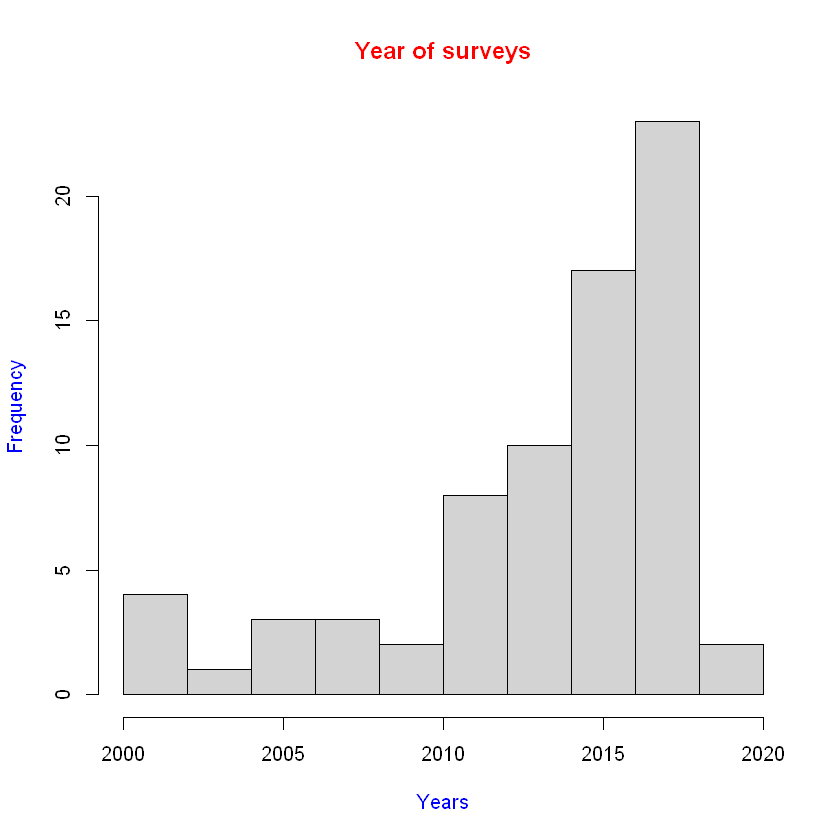
\includegraphics[width=.7\textwidth]{year}
  \caption{Distribution of years of water accessibility variables}
  \label{fig:year}
\end{figure}


\subsection{Cluster analysis}
We selected 22 variables that describe water accessibility of 78 countries around the world \citep{price2019difference}. Next, we used clustering, an unsupervised machine learning method to identify and group water accessibility variables in a large data set to understand and make inferences using R. Clustering ultimately can continue to assist in discovering the water accessibility predictor variables. 

First, we used different clustering algorithms to determine the best clustering results. We tested and clustered using different cluster methodology by utilizing single, average, complete, ward.D, and ward.D2 methods to develop initial clustering dendrogram. Then, we analyzed by determining the best hierarchical relationship of each of the methods by observing the tree diagram itself; more even distributions of each tree are interpreted as optimal clustering methods. We determined that ward.d2 had the evenest distribution, verified through the use of 'NBClust' to determine the best algorithm as well as the best cut or groupings for the clustering methods as shown in \autoref{fig:optimal-clusters}. 

We compared Ward.D2, Ward.D, complete, and k-means algorithm methods to determine the best cuts, and also to confirm that Ward.D2 was the best clustering algorithm method to develop the deprogram tree. The 'NBClust' function was set to determine the best clustering methodology by choosing minimum clustering from 3 to max cuts of 7 and utilized all the indices.NBClust function in R is the 30 algorithm indices for defining the number of clusters and proposes to the user the best clustering design from the different outcomes acquired by diversifying all combinations of many clusters, distance measures, and clustering methods.  Therefore, NBClust determines the best clustering cut for the different methods by determining the mode of the cut numbers which then is called the majority rule.
The majority rule was implemented by the 'NBClust' function for Ward.d2, Ward.D, and the complete algorithm determined that the best clustering cut was four. While, k-means method's majority rule is determined to be three cuts, but we determined that Ward.D2 is the best methodology due to the random nature of the k-mean clustering method. 

Next, we compared the best indices values for different algorithm solving methodology to determine the best cuts to confirm that Ward.D2 is the best methodology. Once again, we determined that Ward.D2 was the best algorithm and learned that the best cut is four trees by analyzing within the different indices values of different algorithm theories. We compared the values by choosing KL, Ratkowsky, and Marriot values to compare what is the best cut for different clustering methods as shown in \autoref{fig:optimal}. 

\begin{table}[h!]
  \centering
  \begin{tabular}{p{1in} p{1in} p{1in}}\toprule
    \bf Methods & \bf KL (clusters) & \bf Value Index \\\midrule
    \texttt{Ward.D2} & 4 & 2.4982 \\\midrule
    \texttt{Ward.D} & 4 & 3.3397 \\\midrule
    \texttt{Complete} & 4 & 3.9093 \\\midrule
     \texttt{K-Means} & 12 & 8.6836  \\\bottomrule
  \end{tabular}
   \centering
  \begin{tabular}{p{1in} p{1in} p{1in}}\toprule
    \bf Methods & \bf Ratkowsky (clusters) & \bf Value Index \\\midrule
    \texttt{Ward.D2} & 4 & 0.2981 \\\midrule
    \texttt{Ward.D} & 4 & 0.2981 \\\midrule
    \texttt{Complete} & 3 & 0.3193 \\\midrule
     \texttt{K-Means} & 3 & 0.2948 \\\bottomrule
  \end{tabular}
   \centering
  \begin{tabular}{p{1in} p{1in} p{1in} p{1in} p{1in}}\toprule
    \bf Methods & \bf Marriot(clusters) & \bf Value Index & \bf Gap & \bf Majority Rule  \\\midrule
    \texttt{Ward.D2} & 4 & 1.54E+40 &  8 & 4 \\\midrule
    \texttt{Ward.D} & 4 & 1.79E+40 & 8 & 4 \\\midrule
    \texttt{Complete} & 4 & 1.77E+40  & 7 & 4 \\\midrule
     \texttt{K-Means} & 4 & 1.54E+40  & \texttt{N/A} & 3  \\\bottomrule
  \end{tabular}
  \caption{Summary of optimal clustering index values (Different Clustering Methods)}
  \label{tab:summary-optimal}
\end{table}

\autoref{tab:summary-optimal} is a rough summary of why Ward.D2 is the best clustering methodology if we go by four cuts. For the KL cluster algorithm, we determined that the best Value index is 2.4982 which is the lowest for the index, and the KL algorithm determines that the lowest value index results from the best cut of four. Also, the Ratkowsky cluster theorem determined that Ward.D2 was the best method for four cuts because the value index was the lowest matching Ward.D at .2981. However, Ward.D is the incomplete version of Ward.D2 where they forgot to square one of the intermediate value in the theorem. Therefore, Ward.D2 is the best clustering method for Ward.D2. Similarly, for the Marriot clustering theorem, Ward.D2 is the best once again due to the Ward.D having the greatest value index which determines that it is the best clustering method. Similar to an explanation from Ratkowsky, Ward.D2 is chosen to be the best method for 4 cuts. \autoref{fig:optimal} shows the visual representation of the explanation by the \autoref{tab:summary-optimal}. 

Lastly, we developed a horizontal dendrogram using R focusing on Ward.D2 methodology for clustering. We also cut the dendrogram in 4 trees as an 'NBClust' analysis as shown in \autoref{fig:dendrogram}. The clustering trees can be further be analyzed and the results and analysis will be discussed in the results and discussion section. 



\subsection{Classification model to explain water accessibility predictors}
%\hl{This is the second phase of the work, which you should hopefully start in January}


\section{Results and Discussion}

\subsection{Exploratory Data Analysis}
A correlation chart was used to assess strong correlations between the 28 numerical variables that may pertain to water accessibility \autoref{fig:cor-basic}. Households with limited water service has the strongest and positive relationship with households possessing a bicycle. Meanwhile, households using an improved water source has the strongest and negative relationship with households using an unimproved water source. This initial finding results indicated that the initial variables are logical and can give us insight into further understanding and the relationship between these variables. 

\begin{figure}[h!]
  \centering
  \includegraphics[width=.7\textwidth]{correlation-basic}
  \caption{Correlation Graph of Numerical Variables}
  \label{fig:cor-basic}
\end{figure}
As we continued to study further upon the correlations of the variables, we used more advanced correlation graphs to determined their p-value, and to see a relationship between different categorical variables is shown in \autoref{fig:cor-plot}, which again indicates a greater detailed comparison between the variables. Households with an improved water source on the premises have a strong relationship with households with basic water service of .84 and a p-value of less than 0.001. Also, we learned and discovered that Households using an unimproved water source have a positive relationship with Households using unprotected well water, Households using an unprotected spring, and Households using surface water with a p-value of less than 0.001 as well. These relationships justify the necessity to research further if the particular water accessibility variables can increase the accessibility of particular water sources to reach universal access to water by 2030, as proposed in the SDGs. 



\begin{figure}[h!]
  \centering
  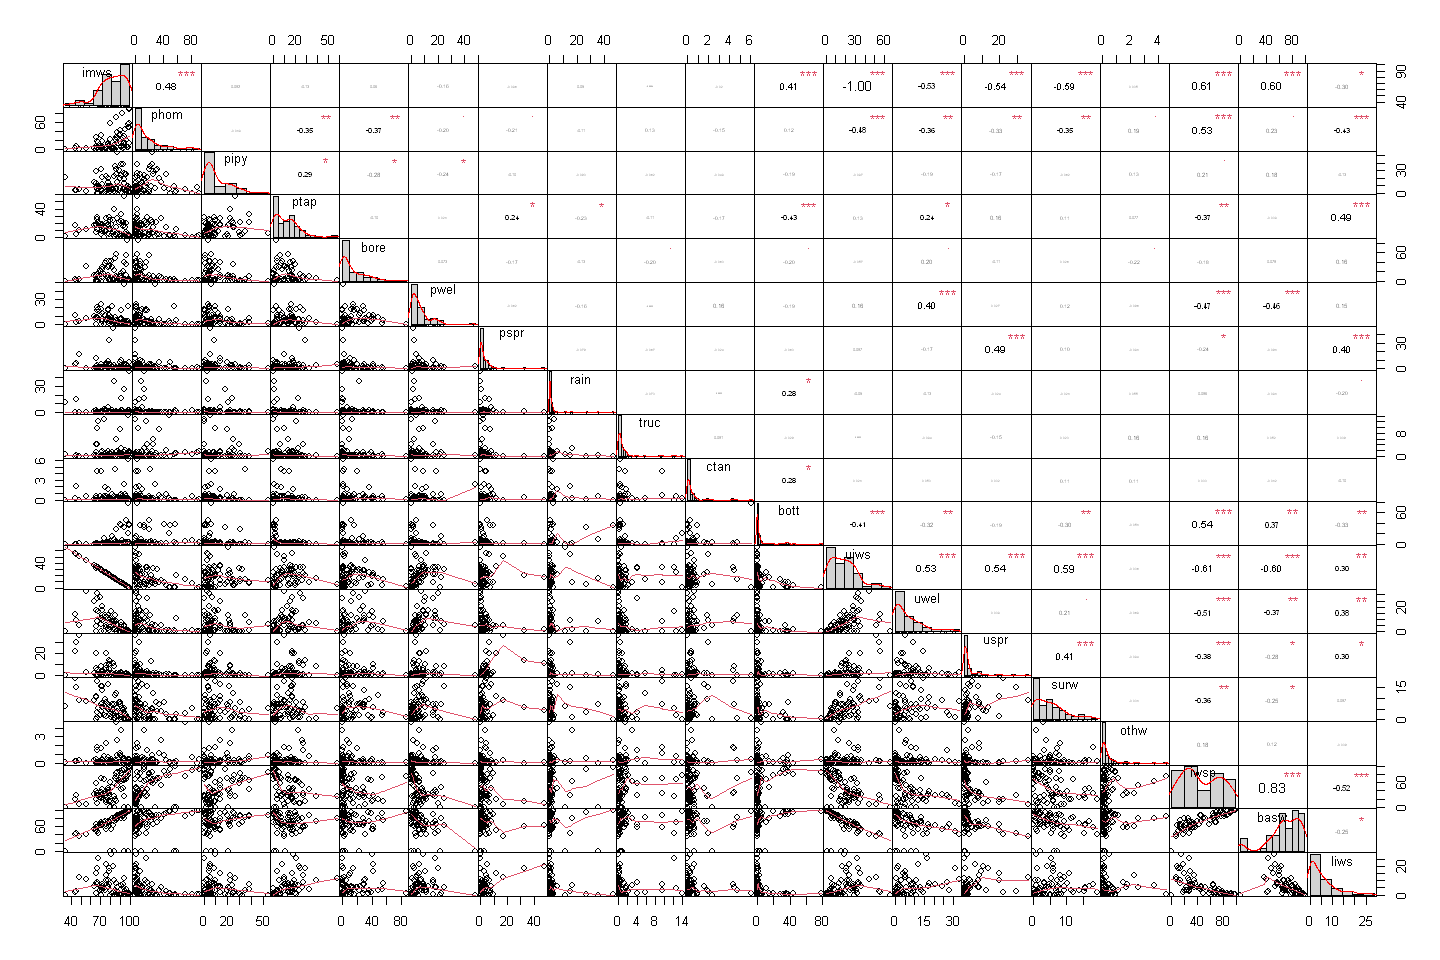
\includegraphics[width=.7\textwidth]{adv-cor-plot}
  \caption{Advanced Correlation Graph of Numerical Variables}
  \label{fig:cor-plot}
\end{figure}

Additionally, we wanted to explore if the modes of transportation variables have any relationship with potential water variables. Therefore, we investigated by developing more correlation plots relating transportation variables with water accessibility variables which are shown in \autoref{fig:transporation-time}, \autoref{fig:transporation-water-one}, \autoref{fig:transporation-water-two}. There is a significant positive relationship between households possessing a private car and households with water on the premises as shown in \autoref{fig:transporation-time}. There is also is a significant negative relationship between households possessing a private car with households with water 30 minutes or less away round trip and households with water more than 30 minutes away round trip with a p-value of less than 0.001. This information is essential to investigate further why this is the global trend. 


\begin{figure}[h!]
  \centering
  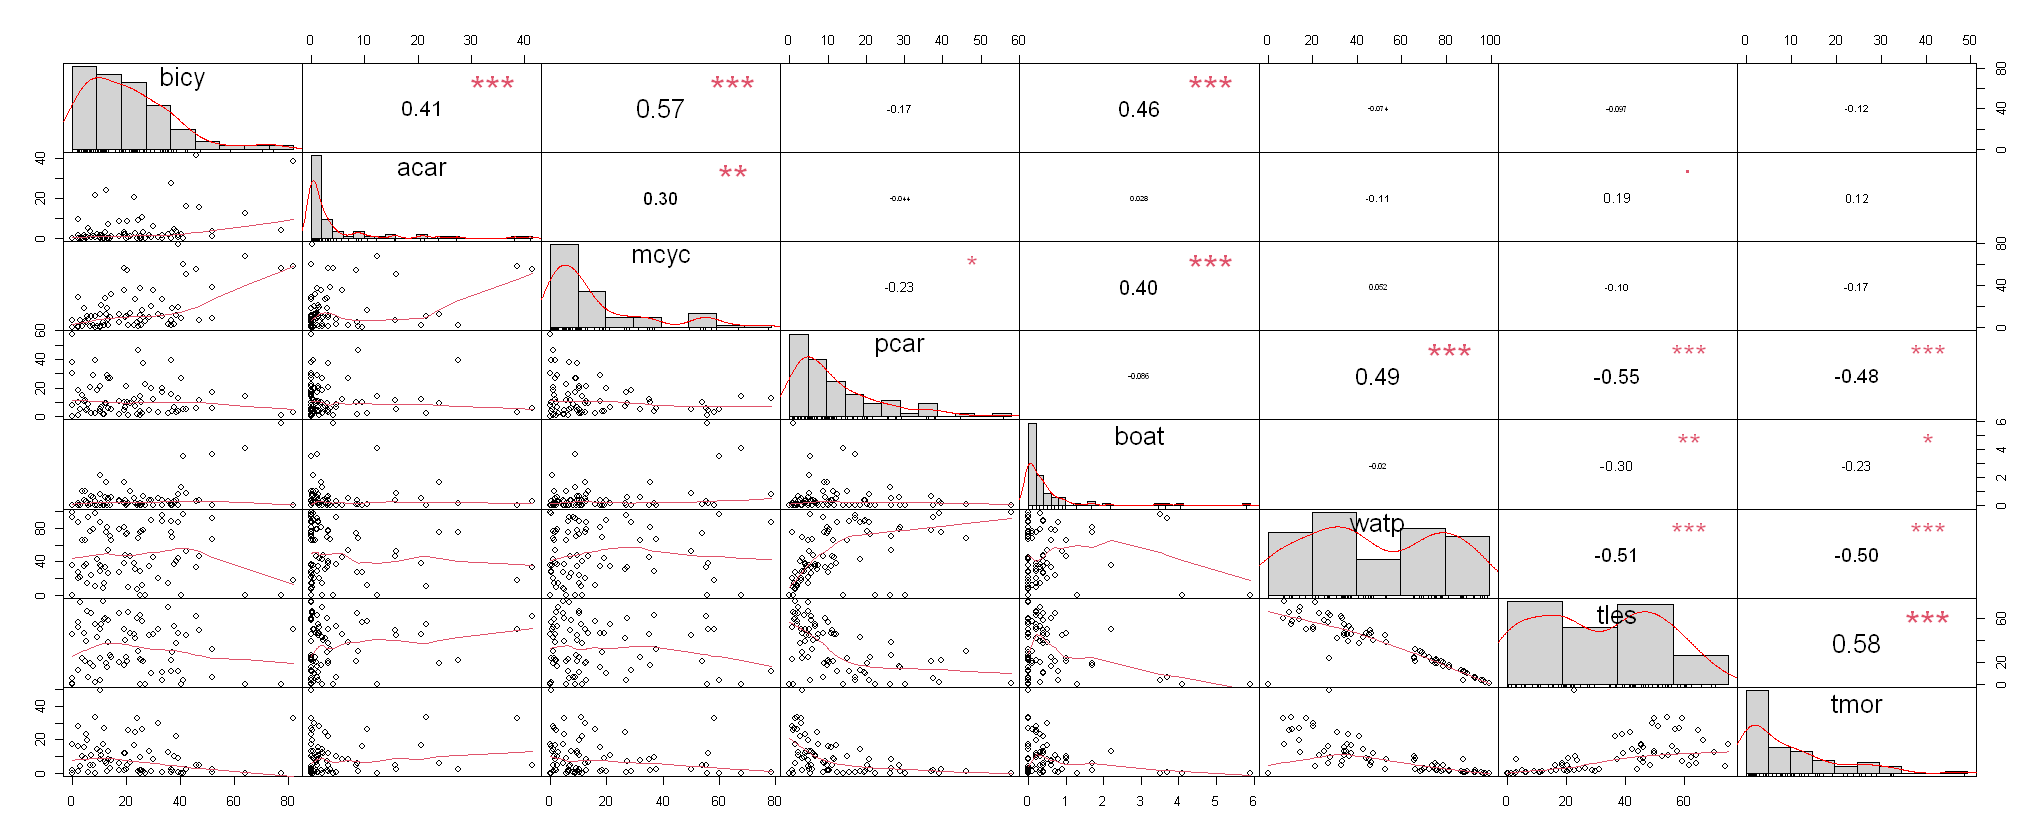
\includegraphics[width=.7\textwidth]{transportation-time}
  \caption{Advanced Correlation Graph of Modes of Transportation and Time}
  \label{fig:transporation-time}
\end{figure}

\autoref{fig:transporation-water-one} shows that Households possessing a motorcycle has a positive correlation with Households using a tube well/borehole and Households using rainwater with a p-value of less than 0.01. Similar to the previous analysis, there is a relationship between a mode of transportation to retrieve potential water sources. \autoref{fig:transporation-water-two} also shows that households possessing an animal-drawn cart have a positive and strong relationship with households using unprotected well water with a p-value of less than 0.001. The results demonstrate that different modes of transportation factor into the accessibility of retrieving water sources on a global scale, therefore, there should be consideration of these variables to increase access to improved water sources. 
\begin{figure}[h!]
  \centering
  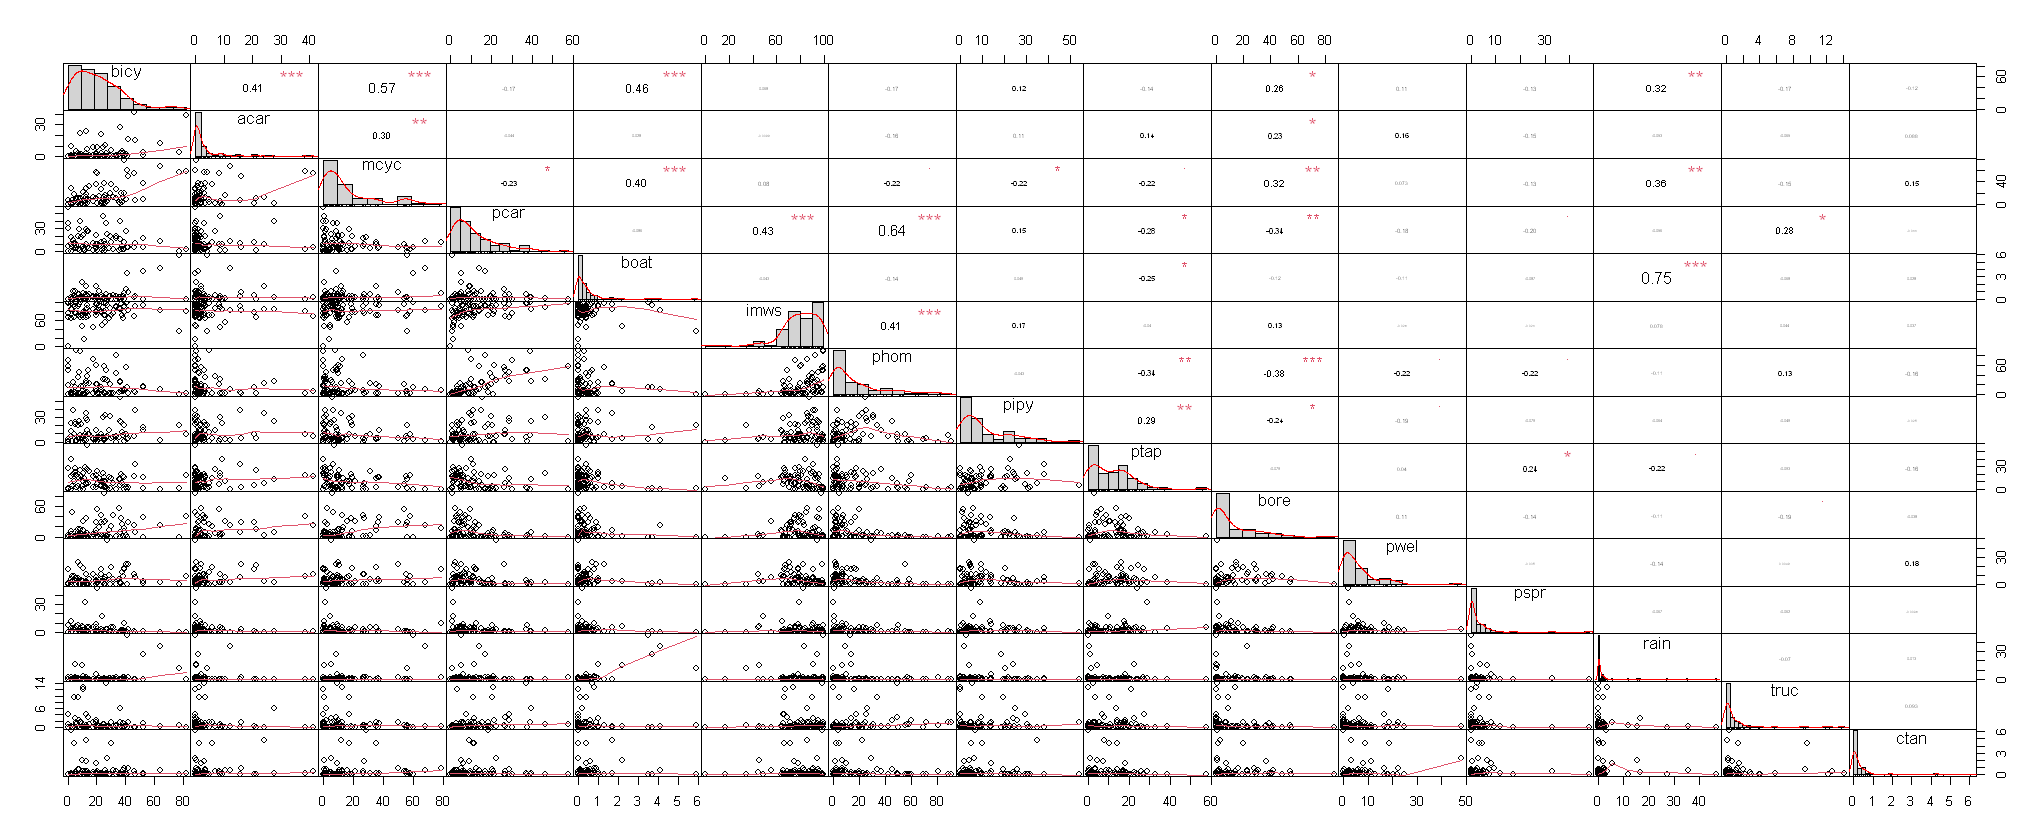
\includegraphics[width=.7\textwidth]{transportation-water-1}
  \caption{Advanced Correlation Graph of Modes of Transportation and Water Resources}
  \label{fig:transporation-water-one}
\end{figure}

\begin{figure}[h!]
  \centering
  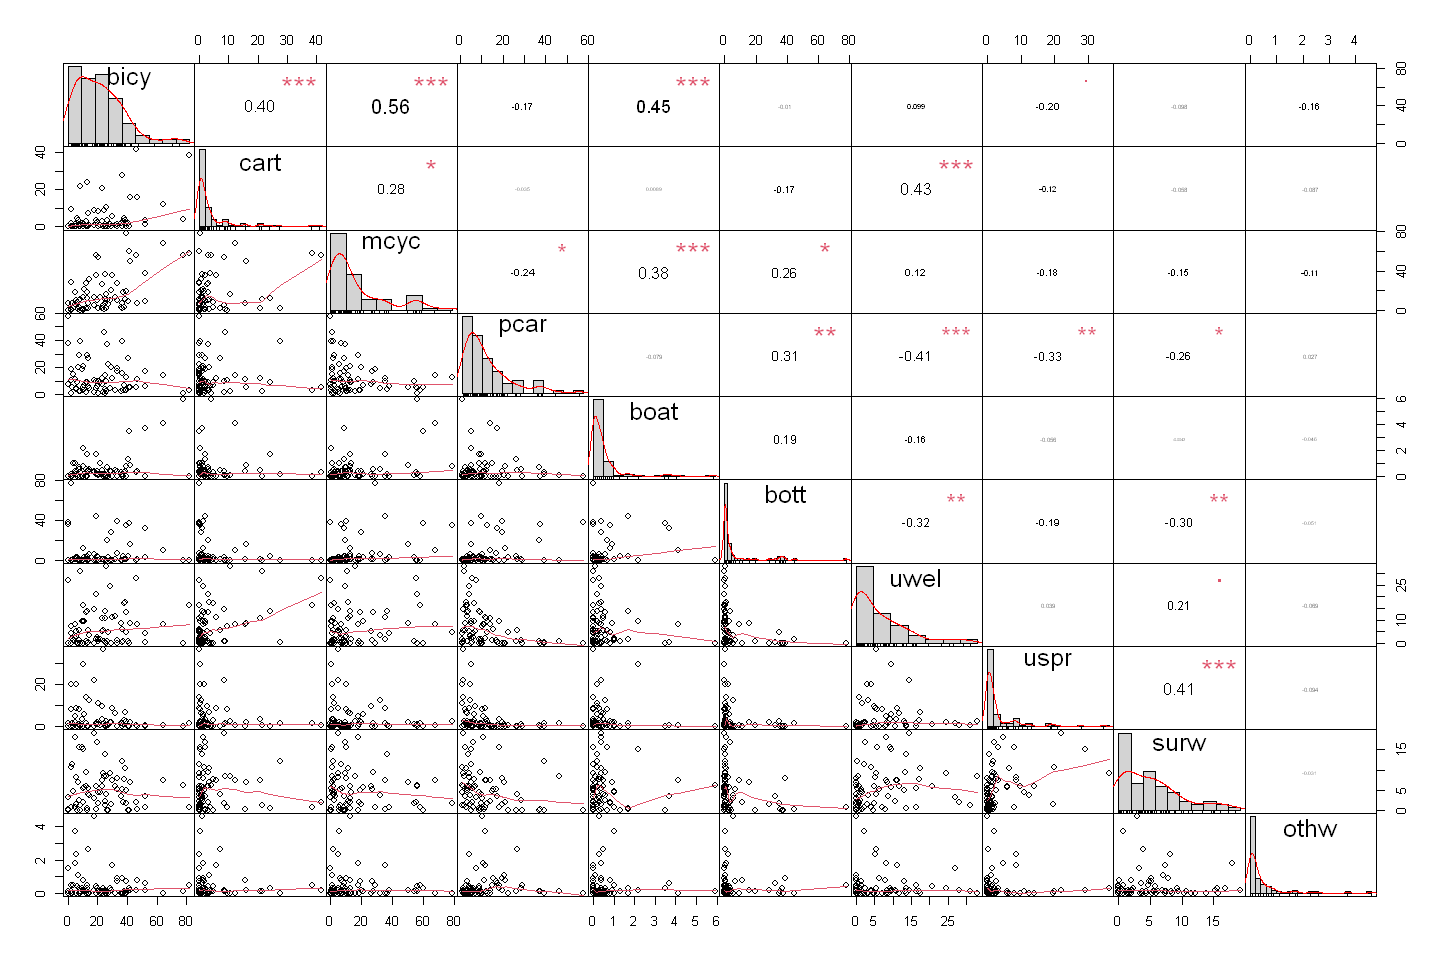
\includegraphics[width=.7\textwidth]{transportation-water-2}
  \caption{Advanced Correlation Graph of Modes of Transportation and Additional Water Resources}
  \label{fig:transporation-water-two}
\end{figure}

There is a problem of people not available to retrieve water quickly and there is a collection burden which is necessary to increase the water quality to improve many people's health and quality of life \citep{cassivi2018access}. These initial findings can allow us to research into what are the major factors of water accessibility for the 76 countries by developing clustering and determining the water accessibility variable predictors. A future study could use the water accessibility variable predictors to implement policies and experiment if it improved water accessibility for the community. This would be a necessary implementation to invest to improve their access to water to reach universal access by 2030.



\subsection{Water accessibility typologies}

NBClust statistic analysis developed and determined four distinct groups. The first cluster group is composed of countries near the equator or in the Sub-Sahara Regions. The analysis of the second group represents countries considered developed or recently industrialized. The third cluster group represents most of the countries in central Africa and may have similar factors as the first cluster group. The fourth cluster group represents most of the countries in the middle east or predominately non-African countries. There are great internally heterogeneous clusters for the 76 distinct countries. The cluster analysis' dendrogram is shown in \autoref{fig:dendrogram}, and the corresponding NBClust curve yielding the optimal four clusters is shown in \autoref{fig:optimal-clusters}, \autoref{fig:optimal}. \autoref{tab:water-cluster} shows the resulting four water accessibility country clusters. The cluster's water accessibility variables are summarized in \autoref{tab:summary-wa}. \autoref{fig:cluster-map} shows the cluster country membership of the water accessibility on a world map.  Through the optimal analysis of the clusters, which indicated the superior grouping of four cuts along with the relevant indicators. 

  
\begin{table}[h!]
  \centering
  \begin{tabular}{p{1in} p{3in} }\toprule
    \bf Clusters & \bf Country Members \\\midrule
    \texttt{A (n=22)} & Afghanistan, Bangladesh, Benin, Burkina Faso, Cameroon, Chad, Ivory Coast, Ghana, Guinea, India, Liberia, Malawi, Mali, Myanmar, Nepal, Niger, Nigeria, Pakistan, Togo, Uganda, Zambia, Zimbabwe  \\\midrule
    \texttt{B (n=14)} & Albania, Armenia, Brazil, Colombia, Egypt, Honduras, Jordan, Kazakhstan, Morocco, Peru, South Africa, Turkey, Ukraine, Uzbekistan  \\\midrule
    \texttt{C (n=20)} & Angola, Burundi, Central African Republic, Congo, Congo Democratic Republic, Eritrea, Eswatini, Ethiopia, Gambia, Haiti, Kenya, Lesotho, Madagascar, Mauritania, Mozambique, Papua New Guinea, Rwanda, Sao Tome and Principe, Sierra Leone, Tanzania  \\\midrule
     \texttt{D (n=22)} & Azerbaijan, Bolivia, Cambodia, Comoros, Dominican Republic, Gabon, Guatemala, Guyana, Indonesia, Kyrgyz Republic, Maldives, Moldova, Namibia, Nicaragua, Paraguay, Philippines, Senegal, Tajikistan, Timor-Leste, Turkmenistan, Vietnam, Yemen  \\\bottomrule
  \end{tabular}
    \caption{Water accessibility country clusters.)}
  \label{tab:water-cluster}
\end{table}

\begin{figure}[h!]
  \centering
  \includegraphics[width=1\textwidth]{cluster-map}
  \caption{Water Accessibility Cluster Map}
  \label{fig:cluster-map}
\end{figure}
	
\begin{figure}[h!]
  \centering
  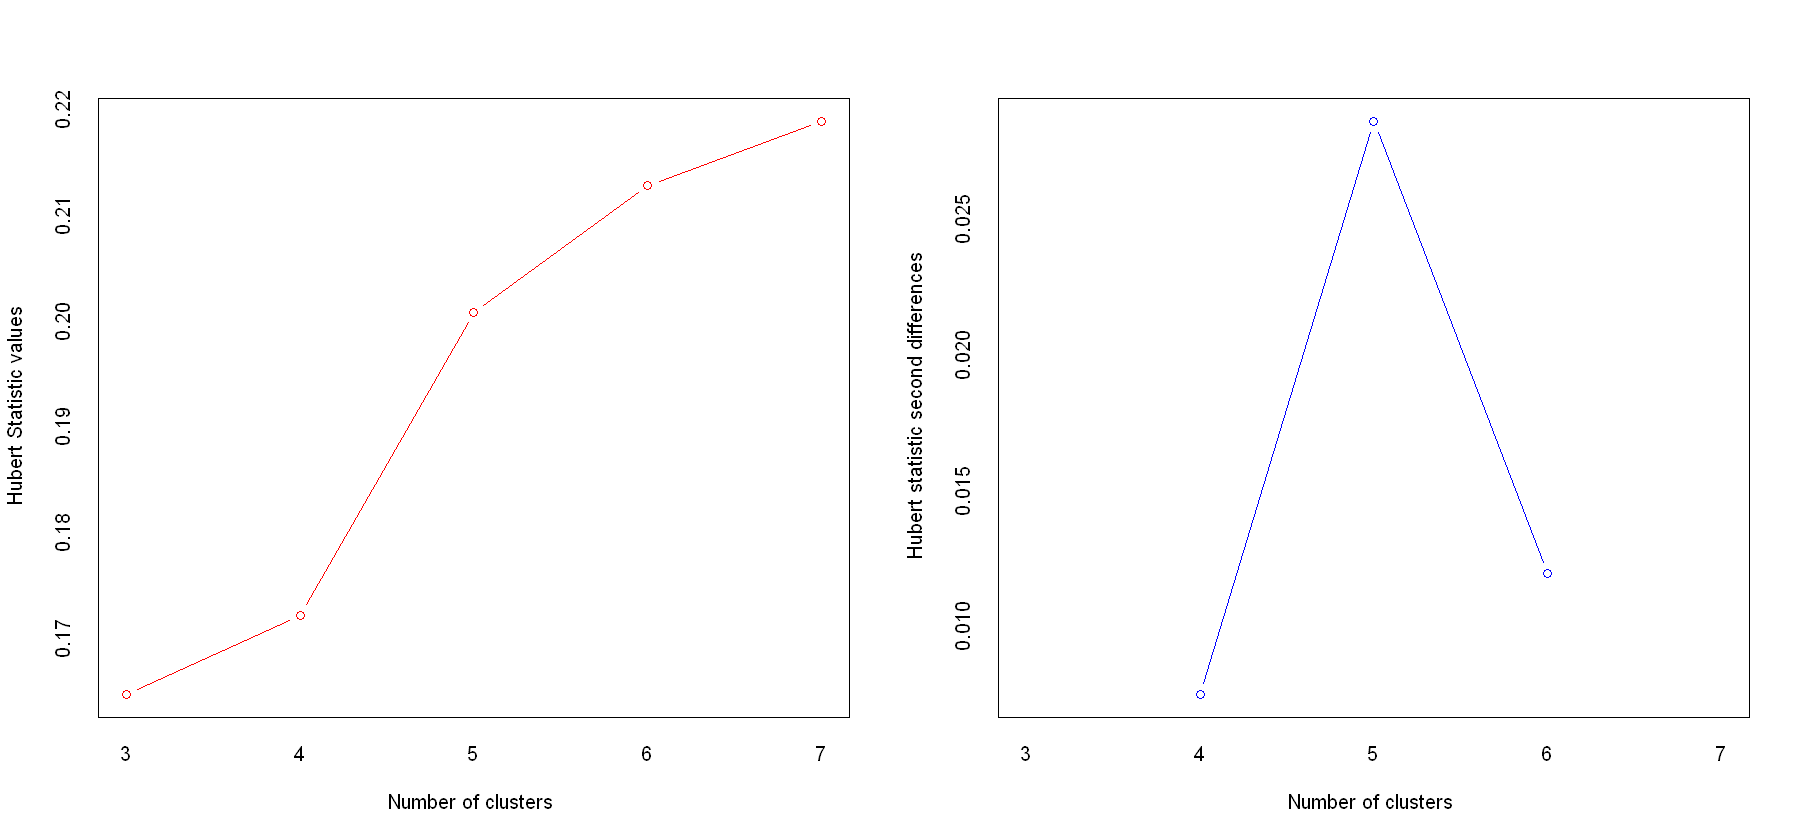
\includegraphics[width=.7\textwidth]{optimal-clusters-ward-d2}
  \caption{Optimal Number of Clusters for Ward.D2}
  \label{fig:optimal-clusters}
\end{figure}

\begin{figure}[h!]
  \centering
  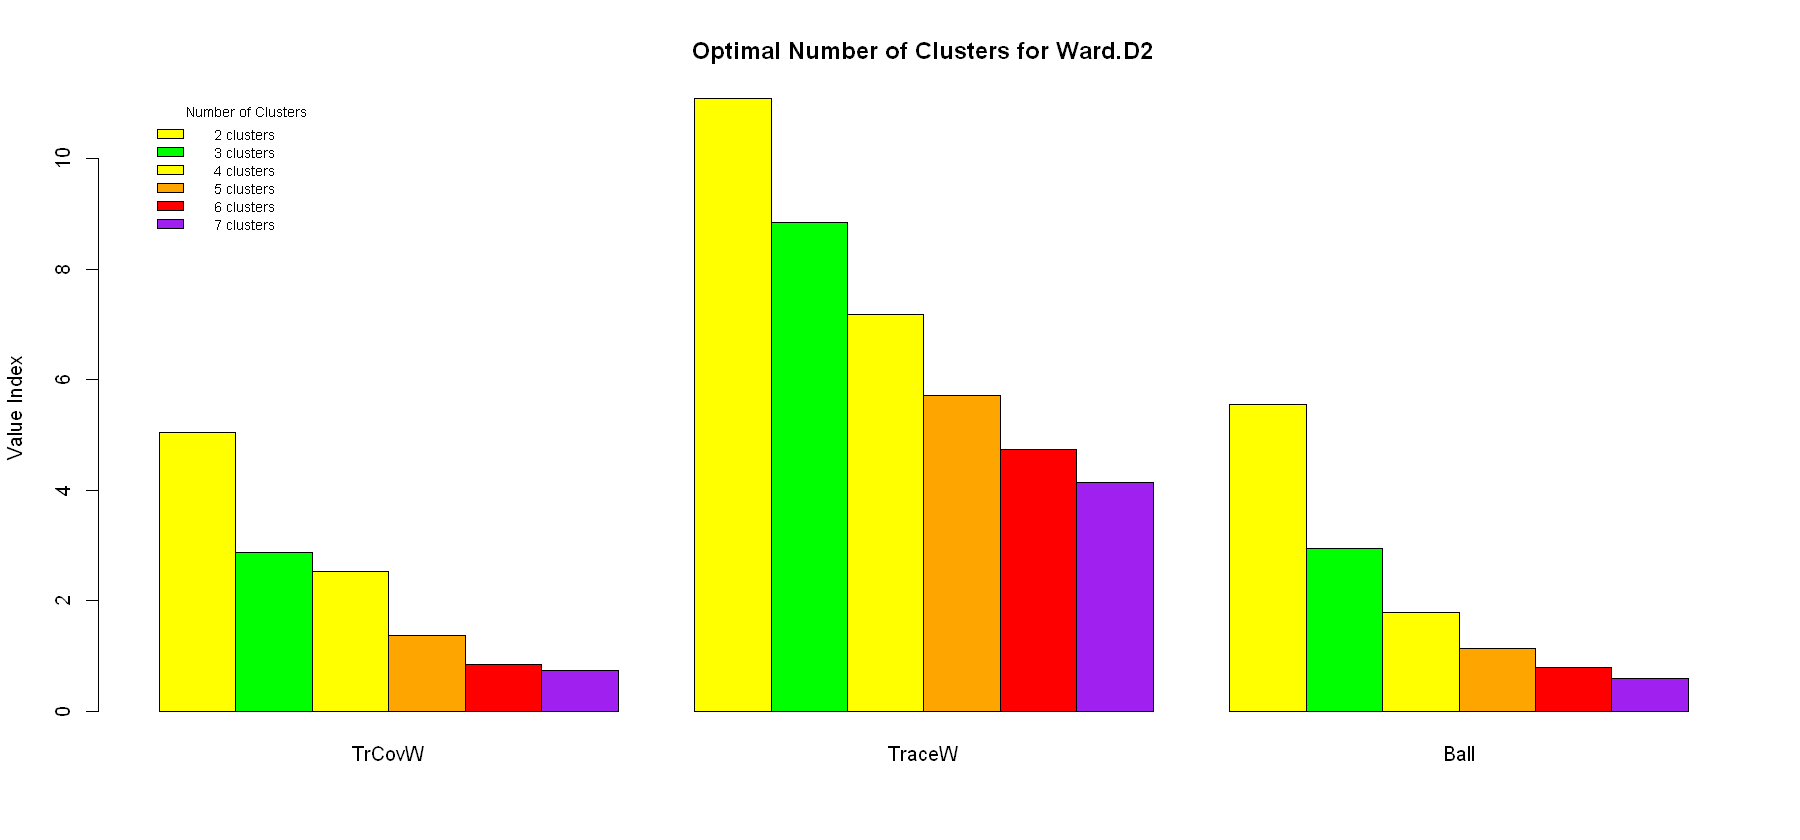
\includegraphics[width=.7\textwidth]{optimal-cuts}
  \caption{Optimal Number of Clusters for Ward.D2}
  \label{fig:optimal}
\end{figure}

\begin{figure}[h!]
  \centering
  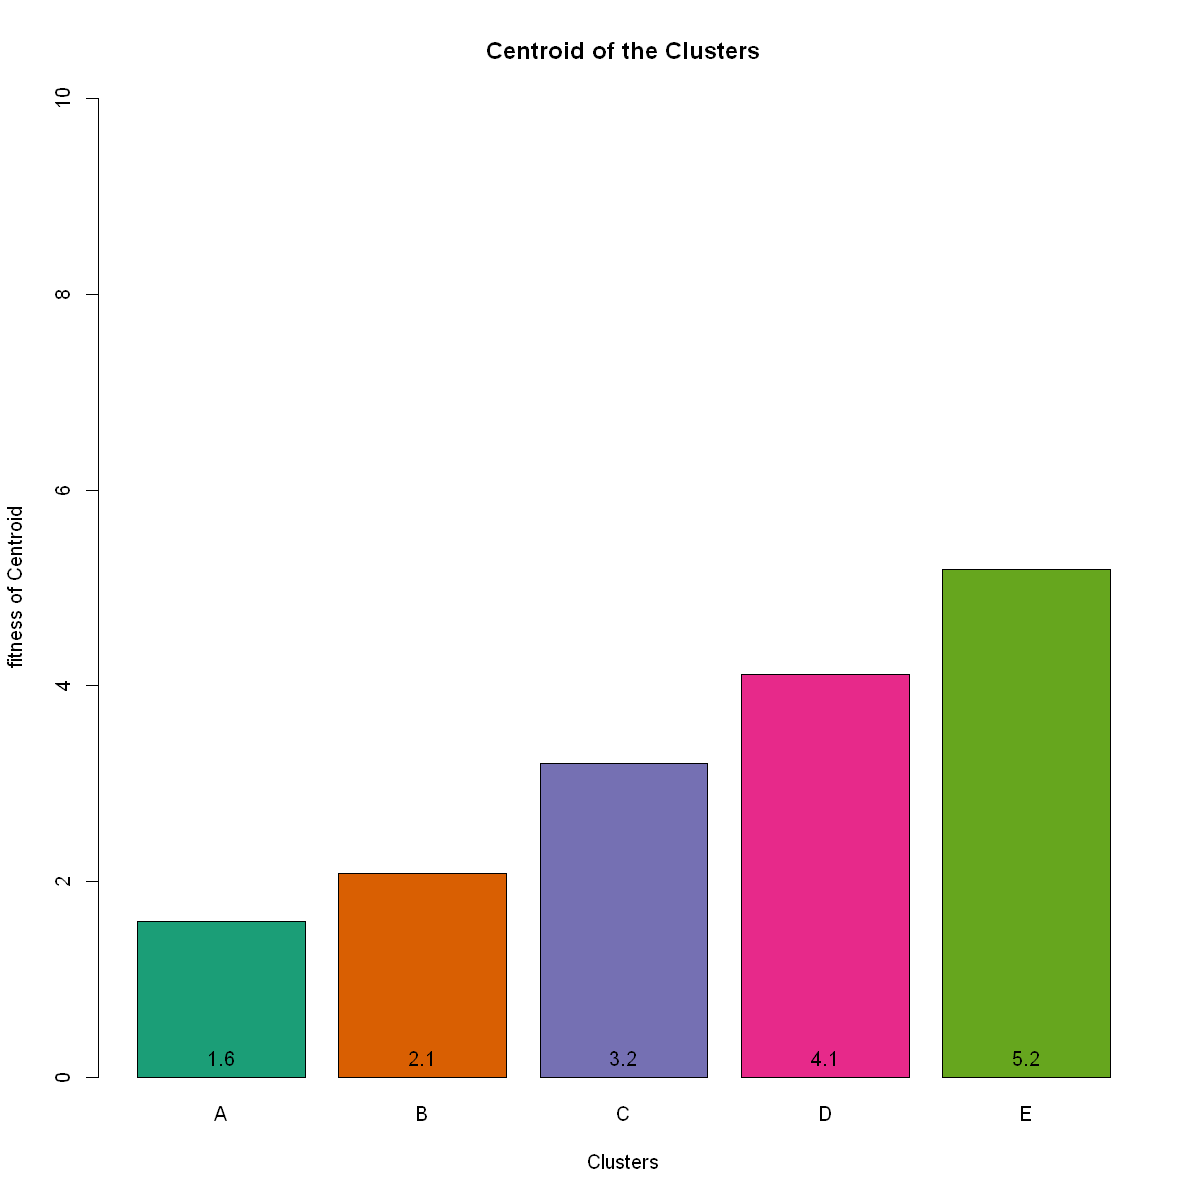
\includegraphics[width=.7\textwidth]{centroid}
  \caption{Centroid of the Four Cluster Groupings}
  \label{fig:centroid}
\end{figure}
\begin{figure}[h!]
  \centering
  \includegraphics[width=1\textwidth]{typology}
  \caption{Cluster Typology Average of Water Accessibility Variables }
  \label{fig:typology}
\end{figure}
\begin{figure}[h!]
\raggedright
  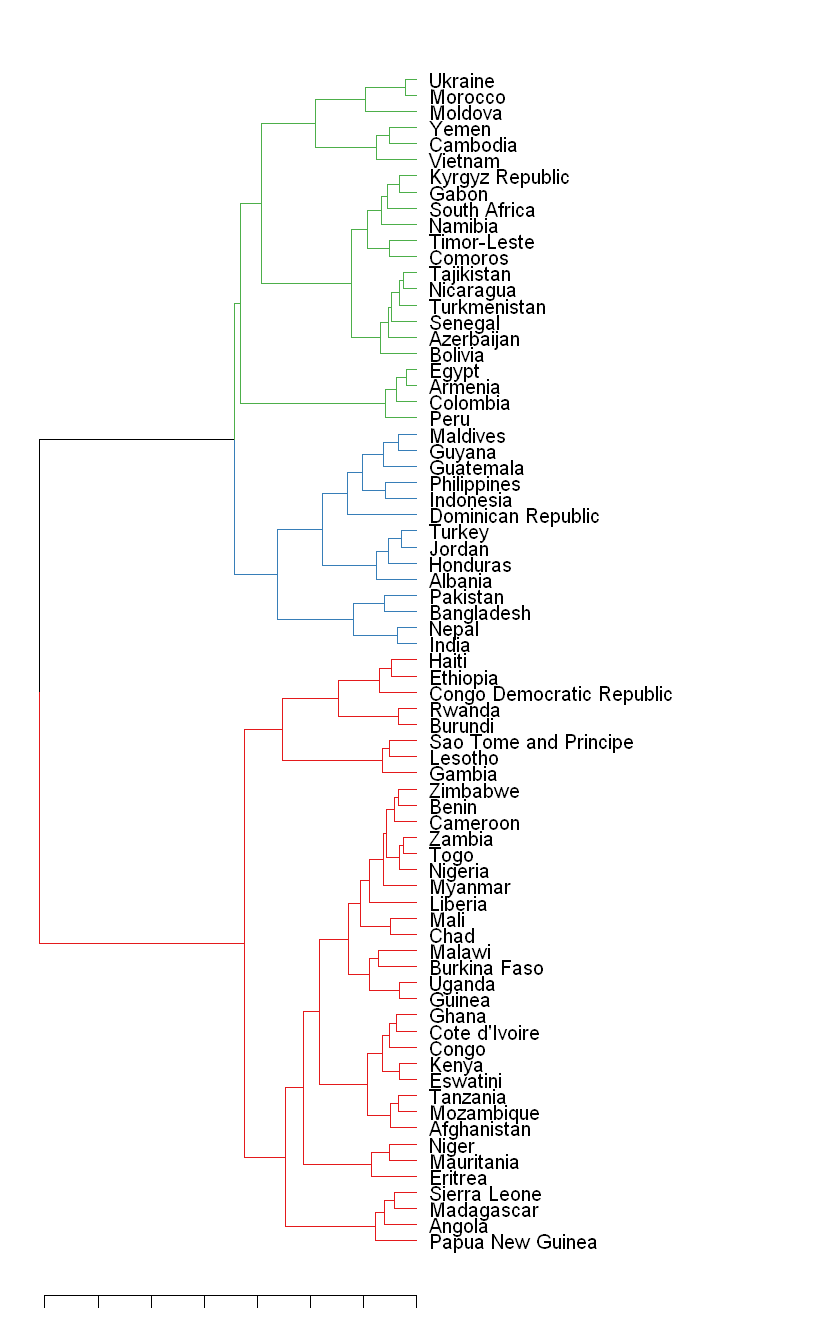
\includegraphics[width=1.15\textwidth]{dendrogram}
  \caption{Cluster Dendrogram with Four Cuts}
  \label{fig:dendrogram}
\end{figure}

\begin{figure}[h!]
  \centering
  \includegraphics[width= 1\textwidth]{spider-plot}
  \caption{Spider Plot of Water Accessibility Variables by Typology}
  \label{fig:spider}
\end{figure}

\subsection{Typology results}
Cluster A consists of 22 countries with major cluster typology factor for Water 30 minutes or less away round trip and Tube well/borehole as shown in \autoref{fig:spider} and \autoref{fig:typology}. Cluster A has countries from Africa and Asia. Cluster A countries are characterized by the high measure of traveling 30 minutes or less to retrieve water and are known to use boreholes as their resource of water. Example country members are Afghanistan, Bangladesh, and Benin. 

Cluster B consists of 14 further advanced and industrialized countries from South America, Europe, Asia, and wealthier African nations. Cluster B countries are categorized by their cluster typology factor for Piped into dwelling as shown in \autoref{fig:spider} and \autoref{fig:typology}. Example country members are Albania, Armenia, and Brazil. 

Cluster C consists of 20 countries mostly in central Africa, some in west Africa and one country in the pacific islands. Cluster C countries are grouped by their cluster typology factor for largest for Water 30 minutes or less away round trip, second largest typology factor of Public tap/standpipe, and third largest typology factor of Water more than 30 minutes away round trip as shown in \autoref{fig:spider} and \autoref{fig:typology}. Example country members are Angola, Burundi, Central African Republic. 

Cluster D consists of 22 geographically dispersed countries. Cluster D countries are categorized by their cluster typology factor for rainwater compared to the other cluster typology. Additionally, the highest factor was Piped into dwelling, but is still lower than the Cluster B as shown in \autoref{fig:spider} and \autoref{fig:typology}. Example country members are Azerbaijan, Bolivia, and Cambodia.  


\section{Discussion}

\section{Conclusion}

\section{Limitation}
%The problem of missing data is relatively common in almost all research and can have a significant effect on the conclusions that can be drawn from the data.

\printbibliography

\end{document}

%%% Local Variables:
%%% mode: latex
%%% TeX-master: t
%%% End:
